%%%%%%%%%%%%%%%%%%%%%%%%%%%%%%%%%%%%%%%%%%%%%%%%%%%%%%%%%%%%%%%%%%%%%%%%%%%%%%
%
% Section file included in main project file using \input{}
%
% Assumes that LaTeX2e macros and packages defined in cg_comp.sty are
%   available
%
%%%%%%%%%%%%%%%%%%%%%%%%%%%%%%%%%%%%%%%%%%%%%%%%%%%%%%%%%%%%%%%%%%%%%%%%%%%%%%

 \section{Classical Guitar Compensation\label{sct:comp}}

 \begin{figure}
  \centering
  \begin{subfigure}[b]{0.45\textwidth}
   \centering
   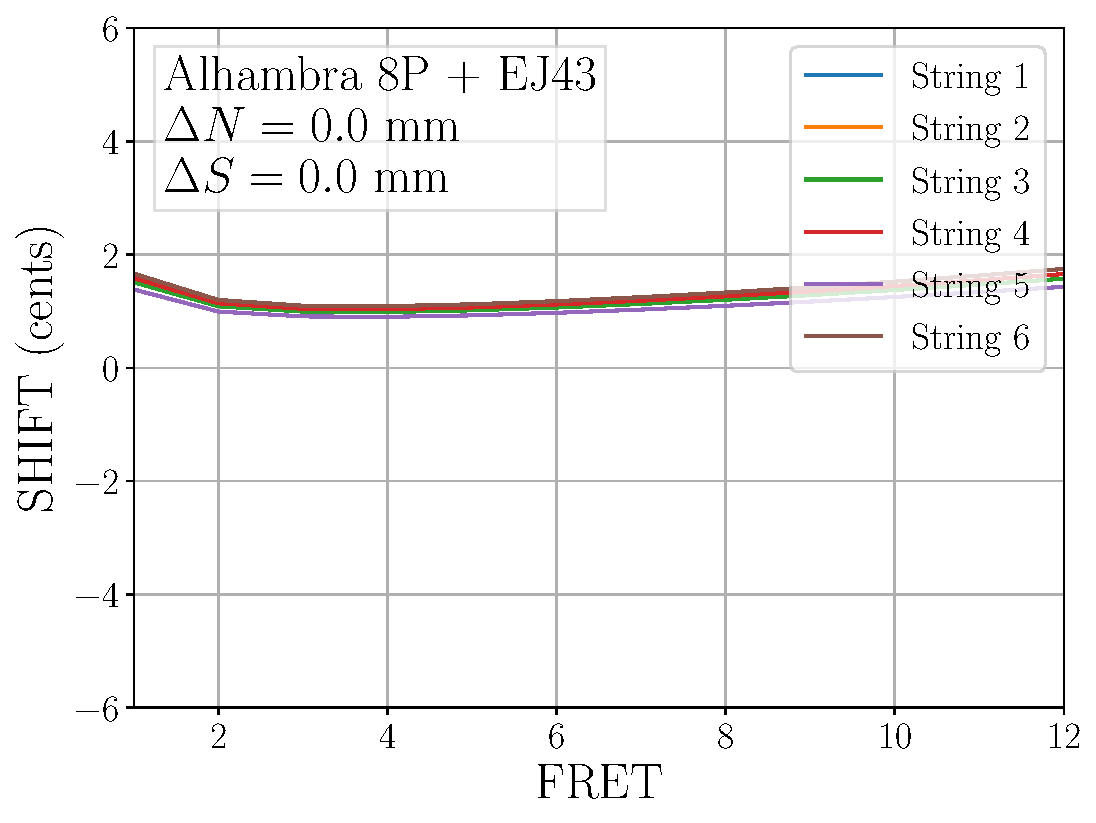
\includegraphics[width=3.25in]{figures/shift_uncompensated}
   \caption{Uncompensated}
   \label{fig:shift_uncompensated}
  \end{subfigure}
  \hspace{0.25in}
  \begin{subfigure}[b]{0.45\textwidth}
   \centering
   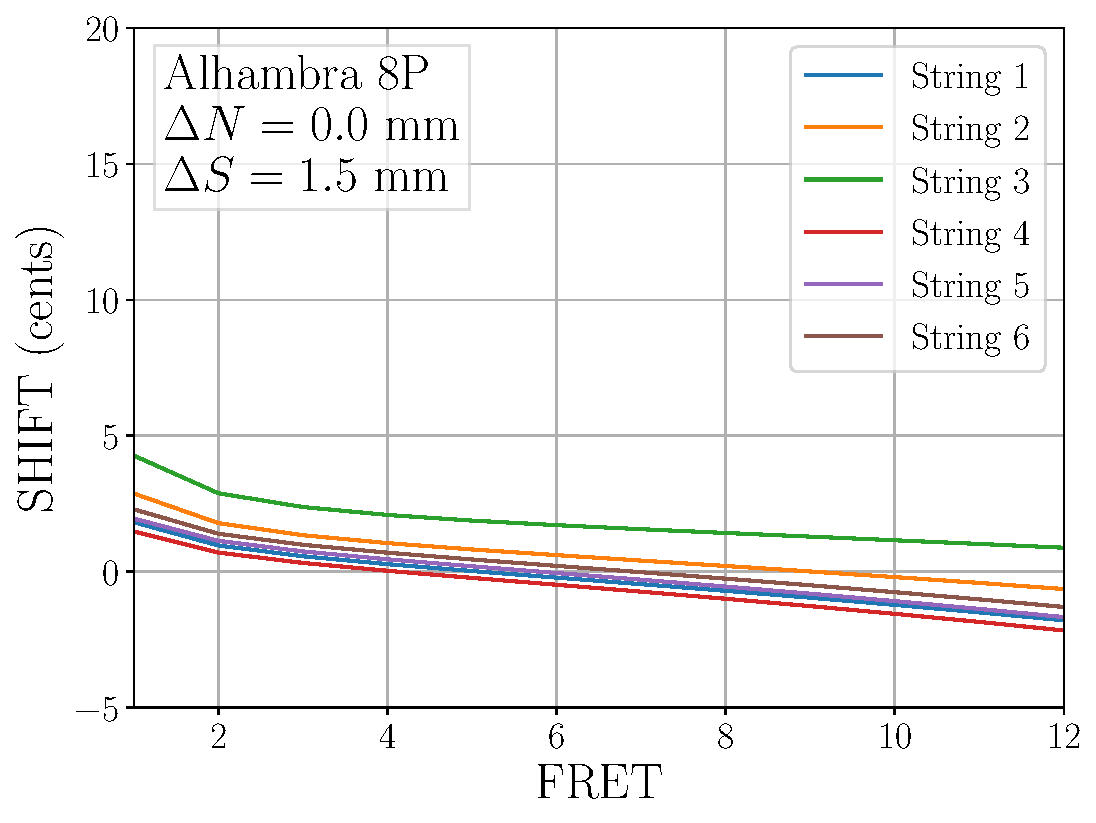
\includegraphics[width=3.25in]{figures/shift_factory}
   \caption{Factory guitar}
   \label{fig:shift_factory}
  \end{subfigure}
  \par\vspace{0.25in}
  \begin{subfigure}[b]{0.45\textwidth}
   \centering
   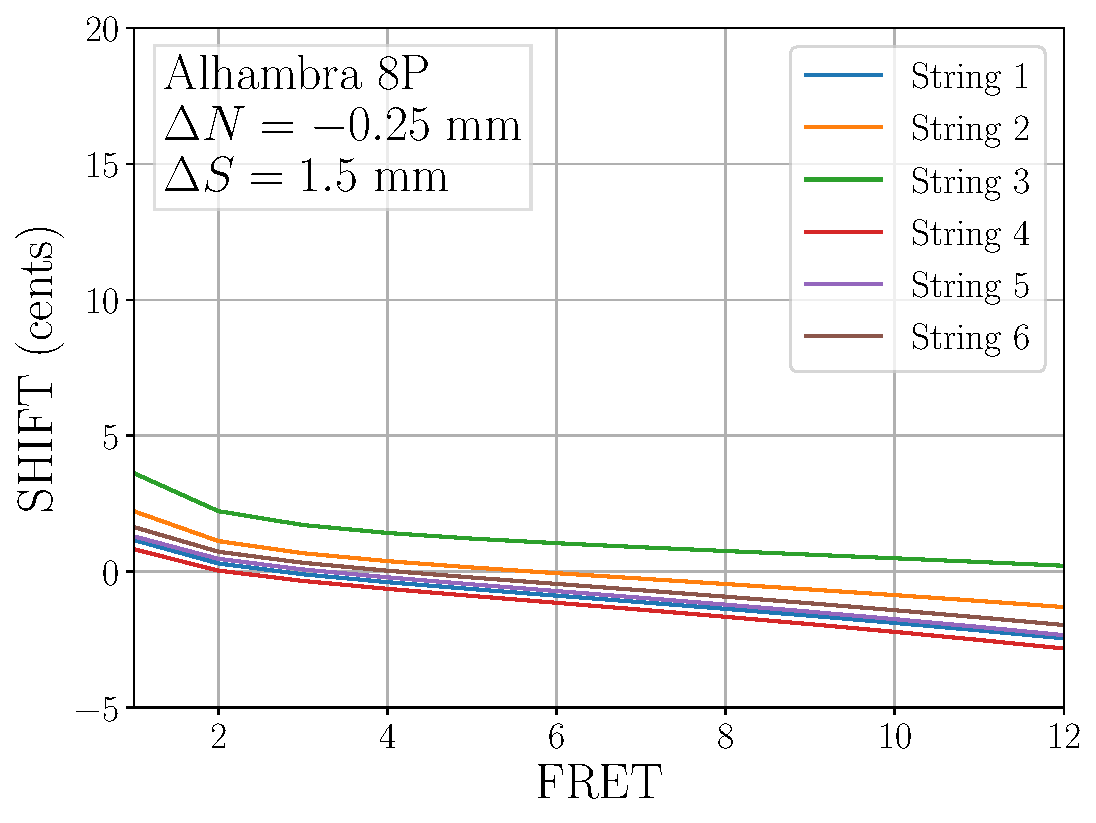
\includegraphics[width=3.25in]{figures/shift_compensated_1}
   \caption{Saddle and nut}
   \label{fig:shift_compensated_1}
  \end{subfigure}
  \hspace{0.25in}
  \begin{subfigure}[b]{0.45\textwidth}
   \centering
   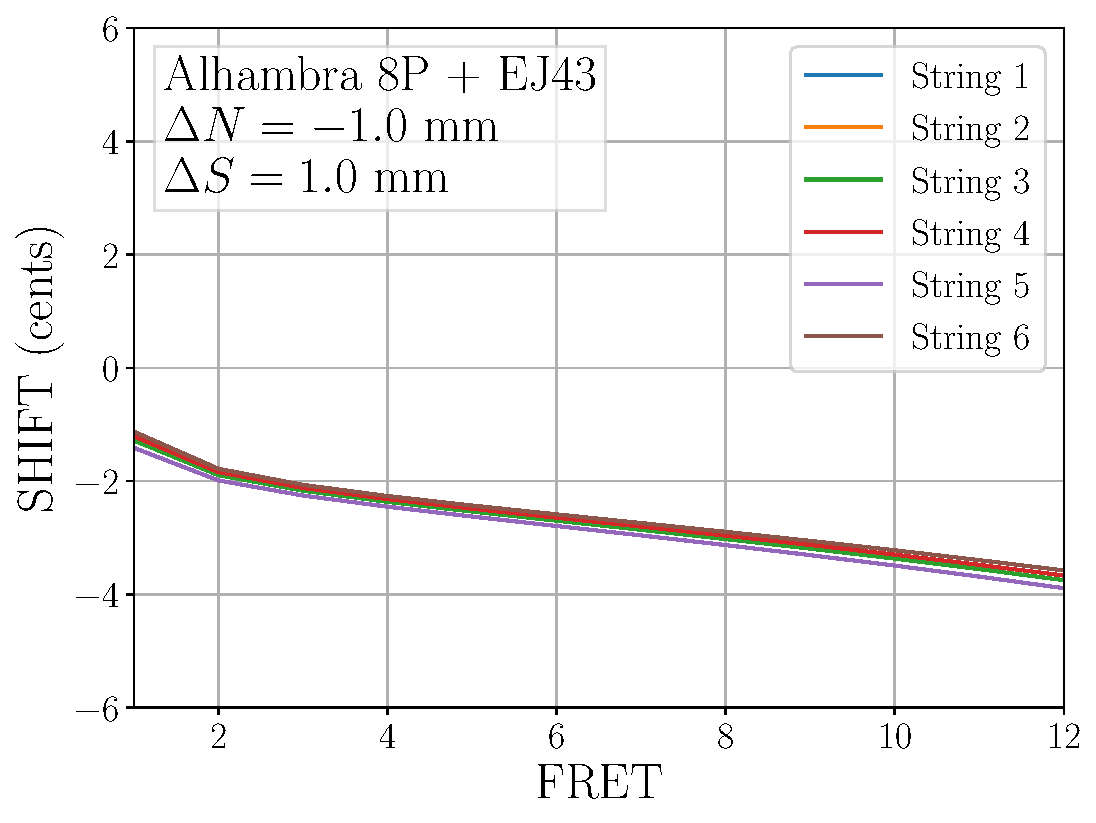
\includegraphics[width=3.25in]{figures/shift_compensated_2}
   \caption{Preserved scale length}
   \label{fig:shift_compensated_2}
  \end{subfigure}
  \caption{\label{fig:compensation} Frequency shift (in cents) for four different strategies of saddle and nut compensation.}
 \end{figure}


